\chapter{Models}\label{models}

\section{Overview}\label{models:overview}

Chapters~\ref{ps} through~\ref{nls} have presented the different
``iterators'' available in DAKOTA.  An iterator iterates on a model in
order to map a set of variables into a set of responses.  This model
may involve a simple mapping involving a single interface, or it may
involve recursions using sub-iterator and sub-models.  These recursion
capabilities were developed in order to provide mechanisms for
``nesting,'' ``layering,'' and ``recasting'' of software components,
which allows the use of these components as building blocks to
accomplish more sophisticated studies, such as surrogate-based
optimization or optimization under uncertainty.  In a nested
relationship, a sub-iterator is executed using its sub-model for every
evaluation of the nested model.  In a layered relationship, on the
other hand, sub-iterators and sub-models are used only for periodic
updates and verifications.  And in a recast relationship, the input
variable and output response definitions in a sub-model are
reformulated in order to support new problem definitions.  In each of
these cases, the sub-model is of arbitrary type, such that model
recursions can be chained together in as long of a sequence as needed
(e.g., layered containing nested contained layered containing single
in Section~\ref{models:ex:ouu:sb}).  Figure~\ref{model:hier} displays
the model class hierarchy from the DAKOTA Developers
Manual~\cite{DevMan}, with derived classes for single models, nested
models, recast models, and two types of surrogate models: data fit and
hierarchical/multifidelity.  A third type of derived surrogate model
supporting reduced-order models (ROM) is planned for future releases.

\begin{figure}
  \centering 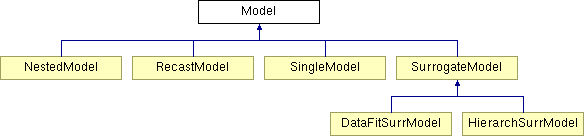
\includegraphics[scale=0.65]{images/classDakota_1_1Model}
  \caption{The DAKOTA model class hierarchy.}  \label{model:hier}
\end{figure}

Section~\ref{models:single} describes single models;
Section~\ref{models:recast} describes recast models;
Section~\ref{models:surrogate} describes surrogate models of the data
fit, multifidelity, and ROM type; and Section~\ref{models:nested}
describes nested models.  Finally, Section~\ref{models:ex} presents
a number of advanced examples demonstrating model recursion.

\section{Single Models}\label{models:single}

The single model is the simplest model type.  It uses a single
interface instance (see Chapter~\ref{interfaces}) to map variables
(see Chapter~\ref{variables}) into responses (see
Chapter~\ref{responses}).  There is no recursion in this case.  Refer
to the Models chapter in the DAKOTA Reference Manual~\cite{RefMan} for
additional information on the single model specification.

\section{Recast Models}\label{models:recast}

The recast model is not directly visible to the user within the input
specification.  Rather, it is used ``behind the scenes'' to recast the
inputs and outputs of a sub-model for the purposes of reformulating
the problem posed to an iterator.  Examples include variable and
response scaling (see Section~\ref{opt:additional:scaling}),
transformations of uncertain variables and associated response
derivatives to employ standardized random variables (see
Sections~\ref{uq:reliability:mpp} and~\ref{uq:expansion:pce}),
multiobjective optimization (see
Section~\ref{opt:additional:multiobjective}), merit functions (see
Section~\ref{sbm:sblm}), and expected improvement/feasibility (see
Sections~\ref{sbm:egm} and~\ref{uq:reliability:global}).  Refer to the
DAKOTA Developers Manual~\cite{DevMan} for additional details on the
mechanics of recasting problem formulations.

\section{Surrogate Models}\label{models:surrogate}

Surrogate models provide an approximation to an original, high
fidelity ``truth'' model.  A number of surrogate model selections are
possible, which are categorized as data fits, multifidelity models,
and reduced-order models.

Each of the surrogate model types supports the use of correction
factors that improve the local accuracy of the surrogate models. The
correction factors force the surrogate models to match the true
function values and possibly true function derivatives at the center
point of each trust region. Currently, DAKOTA supports either zeroth-,
first-, or second-order accurate correction methods, each of which can
be applied using either an additive, multiplicative, or combined
correction function. For each of these correction approaches, the
correction is applied to the surrogate model and the corrected model
is then interfaced with whatever algorithm is being employed.  The
default behavior is that no correction factor is applied.

The simplest correction approaches are those that enforce consistency
in function values between the surrogate and original models at a
single point in parameter space through use of a simple scalar offset
or scaling applied to the surrogate model.  First-order corrections
such as the first-order multiplicative correction (also known as beta
correction~\cite{Cha93}) and the first-order additive
correction~\cite{Lew00} also enforce consistency in the gradients and
provide a much more substantial correction capability that is
sufficient for ensuring provable convergence in SBO algorithms (see
Section~\ref{sbm:sblm}).  SBO convergence rates can be further
accelerated through the use of second-order corrections which also
enforce consistency in the Hessians~\cite{Eld04}, where the
second-order information may involve analytic, finite-difference, or
quasi-Newton Hessians.

Correcting surrogate models with additive corrections involves
\begin{equation}
\hat{f_{hi_{\alpha}}}({\bf x}) = f_{lo}({\bf x}) + \alpha({\bf x}) 
\label{eq:correct_val_add}
\end{equation}
where multifidelity notation has been adopted for clarity.  For
multiplicative approaches, corrections take the form
\begin{equation}
\hat{f_{hi_{\beta}}}({\bf x}) = f_{lo}({\bf x}) \beta({\bf x})
\label{eq:correct_val_mult}
\end{equation}
where, for local corrections, $\alpha({\bf x})$ and $\beta({\bf x})$
are first or second-order Taylor series approximations to the exact
correction functions:
\begin{eqnarray}
\alpha({\bf x}) & = & A({\bf x_c}) + \nabla A({\bf x_c})^T 
({\bf x} - {\bf x_c}) + \frac{1}{2} ({\bf x} - {\bf x_c})^T 
\nabla^2 A({\bf x_c}) ({\bf x} - {\bf x_c}) \label{eq:taylor_a} \\
\beta({\bf x})  & = & B({\bf x_c}) + \nabla B({\bf x_c})^T 
({\bf x} - {\bf x_c}) + \frac{1}{2} ({\bf x} - {\bf x_c})^T \nabla^2 
B({\bf x_c}) ({\bf x} - {\bf x_c}) \label{eq:taylor_b}
\end{eqnarray}
where the exact correction functions are
\begin{eqnarray}
A({\bf x}) & = & f_{hi}({\bf x}) - f_{lo}({\bf x})       \label{eq:exact_A} \\
B({\bf x}) & = & \frac{f_{hi}({\bf x})}{f_{lo}({\bf x})} \label{eq:exact_B}
\end{eqnarray}
Refer to \cite{Eld04} for additional details on the derivations.

A combination of additive and multiplicative corrections can provide
for additional flexibility in minimizing the impact of the correction
away from the trust region center.  In other words, both additive and
multiplicative corrections can satisfy local consistency, but through
the combination, global accuracy can be addressed as well.  This
involves a convex combination of the additive and multiplicative
corrections:
\begin{equation}
\hat{f_{hi_{\gamma}}}({\bf x}) = \gamma \hat{f_{hi_{\alpha}}}({\bf x}) +
(1 - \gamma) \hat{f_{hi_{\beta}}}({\bf x}) \label{eq:combined_form}
\end{equation}
where $\gamma$ is calculated to satisfy an additional matching
condition, such as matching values at the previous design iterate.

%It should be noted that in both first order correction methods, the
%function $\hat{f}(x)$ matches the function value and gradients of
%$f_{t}(x)$ at $x=x_{c}$. This property is necessary in proving that
%the first order-corrected SBO algorithms are provably convergent to a
%local minimum of $f_{t}(x)$.  However, the first order correction
%methods are significantly more expensive than the zeroth order
%correction methods, since the first order methods require computing
%both $\nabla f_{t}(x_{c})$ and $\nabla f_{s}(x_{c})$.  When the SBO
%strategy is used with either of the zeroth order correction methods,
%or with no correction method, convergence is not guaranteed to a local
%minimum of $f_{t}(x)$. That is, the SBO strategy becomes a heuristic
%optimization algorithm. From a mathematical point of view this is
%undesirable, but as a practical matter, the heuristic variants of SBO
%are often effective in finding local minima.

%\emph{Usage guidelines:}
%\begin{itemize}
%\item Both the \texttt{additive zeroth\_order} and
%  \texttt{multiplicative zeroth\_order} correction methods are
%  ``free'' since they use values of $f_{t}(x_{c})$ that are normally
%  computed by the SBO strategy.
%
%\item The use of either the \texttt{additive first\_order} method or
%  the \texttt{multiplicative first\_order} method does not necessarily
%  improve the rate of convergence of the SBO algorithm.
%
%\item When using the first order correction methods, the
%  \texttt{TRUE\_FCN\_GRAD} response keywords must be modified (see
%  bottom of Figure~\ref{sbm:sblm_rosen}) to allow either analytic or
%  numerical gradients to be computed. This provides the gradient data
%  needed to compute the correction function.
%
%\item For many computationally expensive engineering optimization
%  problems, gradients often are too expensive to obtain or are
%  discontinuous (or may not exist at all). In such cases the heuristic
%  SBO algorithm has been an effective approach at identifying optimal
%  designs~\cite{Giu02}.
%\end{itemize}

\subsection{Data Fit Surrogate Models}\label{models:surrogate:datafit}

A surrogate of the {\em data fit} type is a non-physics-based
approximation typically involving interpolation or regression of a set
of data generated from the original model.  Data fit surrogates can be
further characterized by the number of data points used in the fit,
where a local approximation (e.g., first or second-order Taylor
series) uses data from a single point, a multipoint approximation
(e.g., two-point exponential approximations (TPEA) or two-point
adaptive nonlinearity approximations (TANA)) uses a small number of
data points often drawn from the previous iterates of a particular
algorithm, and a global approximation (e.g., polynomial response
surfaces, kriging, neural networks, radial basis functions, splines)
uses a set of data points distributed over the domain of interest,
often generated using a design of computer experiments.

DAKOTA contains several types of surface fitting methods that can be
used with optimization and uncertainty quantification methods and
strategies such as surrogate-based optimization and optimization under
uncertainty. These are: polynomial models (linear, quadratic, and
cubic), first-order Taylor series expansion, kriging spatial
interpolation, artificial neural networks, multivariate adaptive
regression splines, radial basis functions, and moving least squares. 
With the exception of Taylor series methods, all of the above methods 
listed in the previous sentence are accessed in DAKOTA through the 
Surfpack library.  All of these surface fitting methods can be
applied to problems having an arbitrary number of design parameters.
However, surface fitting methods usually are practical only for
problems where there are a small number of parameters (e.g., a maximum
of somewhere in the range of 30-50 design parameters). The
mathematical models created by surface fitting methods have a variety
of names in the engineering community. These include surrogate models,
meta-models, approximation models, and response surfaces. For this
manual, the terms surface fit model and surrogate model are used.

The data fitting methods in DAKOTA include software developed by
Sandia researchers and by various researchers in the academic
community.

\subsubsection{Procedures for Surface Fitting}\label{models:surf:procedures}

The surface fitting process consists of three steps: (1) selection of
a set of design points, (2) evaluation of the true response quantities
(e.g., from a user-supplied simulation code) at these design points,
and (3) using the response data to solve for the unknown coefficients
(e.g., polynomial coefficients, neural network weights, kriging
correlation factors) in the surface fit model. In cases where there is
more than one response quantity (e.g., an objective function plus one
or more constraints), then a separate surface is built for each
response quantity. Currently, the surface fit models are built using
only 0$^{\mathrm{th}}$-order information (function values only), although
extensions to using higher-order information (gradients and Hessians)
are possible. Each surface fitting method employs a different
numerical method for computing its internal coefficients. For example,
the polynomial surface uses a least-squares approach that employs a
singular value decomposition to compute the polynomial coefficients,
whereas the kriging surface uses Maximum Likelihood Estimation to
compute its correlation coefficients. More information on the
numerical methods used in the surface fitting codes is provided in the
DAKOTA Developers Manual~\cite{DevMan}.

The set of design points that is used to construct a surface fit model
is generated using either the DDACE software package~\cite{TonXX} or the
LHS software package~\cite{Ima84}. These packages provide a variety of
sampling methods including Monte Carlo (random) sampling, Latin
hypercube sampling, orthogonal array sampling, central composite
design sampling, and Box-Behnken sampling. More information on these
software packages is provided in Chapter~\ref{dace}.

\subsubsection{Taylor Series}\label{models:surf:taylor}

The Taylor series model is purely a local approximation method. That
is, it provides local trends in the vicinity of a single point in
parameter space. The first-order Taylor series expansion is:
\begin{equation}
\hat{f}({\bf x}) \approx f({\bf x}_0) + \nabla_{\bf x} f({\bf x}_0)^T 
({\bf x} - {\bf x}_0) \label{eq:taylor1}
\end{equation}
and the second-order expansion is:
\begin{equation}
\hat{f}({\bf x}) \approx f({\bf x}_0) + \nabla_{\bf x} f({\bf x}_0)^T 
({\bf x} - {\bf x}_0) + \frac{1}{2} ({\bf x} - {\bf x}_0)^T 
\nabla^2_{\bf x} f({\bf x}_0) ({\bf x} - {\bf x}_0) \label{eq:taylor2}
\end{equation}

where ${\bf x}_0$ is the expansion point in $n$-dimensional parameter
space and $f({\bf x}_0)$, $\nabla_{\bf x} f({\bf x}_0)$, and
$\nabla^2_{\bf x} f({\bf x}_0)$ are the computed response value,
gradient, and Hessian at the expansion point, respectively.  As
dictated by the responses specification used in building the local
surrogate, the gradient may be analytic or numerical and the Hessian
may be analytic, numerical, or based on quasi-Newton secant updates.

In general, the Taylor series model is accurate only in the region of
parameter space that is close to ${\bf x}_0$ . While the accuracy is
limited, the first-order Taylor series model reproduces the correct
value and gradient at the point $\mathbf{x}_{0}$, and the second-order
Taylor series model reproduces the correct value, gradient, and
Hessian. This consistency is useful in provably-convergent
surrogate-based optimization. The other surface fitting methods do not
use gradient information directly in their models, and these methods
rely on an external correction procedure in order to satisfy the
consistency requirements of provably-convergent SBO.

\subsubsection{Two Point Adaptive Nonlinearity Approximation}\label{models:surf:tana}

The TANA-3 method~\cite{Xu98} is a multipoint approximation method
based on the two point exponential approximation~\cite{Fad90}. This
approach involves a Taylor series approximation in intermediate
variables where the powers used for the intermediate variables are
selected to match information at the current and previous expansion
points.  The form of the TANA model is:

\begin{equation}
\hat{f}({\bf x}) \approx f({\bf x}_2) + \sum_{i=1}^n 
\frac{\partial f}{\partial x_i}({\bf x}_2) \frac{x_{i,2}^{1-p_i}}{p_i} 
(x_i^{p_i} - x_{i,2}^{p_i}) + \frac{1}{2} \epsilon({\bf x}) \sum_{i=1}^n 
(x_i^{p_i} - x_{i,2}^{p_i})^2 \label{eq:tana_f}
\end{equation}

where $n$ is the number of variables and:

\begin{eqnarray}
p_i & = & 1 + \ln \left[ \frac{\frac{\partial f}{\partial x_i}({\bf x}_1)}
{\frac{\partial f}{\partial x_i}({\bf x}_2)} \right] \left/ 
\ln \left[ \frac{x_{i,1}}{x_{i,2}} \right] \right. \label{eq:tana_pi} \\
\epsilon({\bf x}) & = & \frac{H}{\sum_{i=1}^n (x_i^{p_i} - x_{i,1}^{p_i})^2 + 
\sum_{i=1}^n (x_i^{p_i} - x_{i,2}^{p_i})^2} \label{eq:tana_eps} \\
H & = & 2 \left[ f({\bf x}_1) - f({\bf x}_2) - \sum_{i=1}^n 
\frac{\partial f}{\partial x_i}({\bf x}_2) \frac{x_{i,2}^{1-p_i}}{p_i} 
(x_{i,1}^{p_i} - x_{i,2}^{p_i}) \right] \label{eq:tana_H}
\end{eqnarray}

and ${\bf x}_2$ and ${\bf x}_1$ are the current and previous expansion
points.  Prior to the availability of two expansion points, a
first-order Taylor series is used.

\subsubsection{Linear, Quadratic, and Cubic Polynomial Models}\label{models:surf:polynomial}

Linear, quadratic, and cubic polynomial models are available in
DAKOTA. The form of the linear polynomial model is

\begin{equation}
  \hat{f}(\mathbf{x}) \approx c_{0}+\sum_{i=1}^{n}c_{i}x_{i}
  \label{models:surf:equation01}
\end{equation}

the form of the quadratic polynomial model is:

\begin{equation}
  \hat{f}(\mathbf{x}) \approx c_{0}+\sum_{i=1}^{n}c_{i}x_{i}
  +\sum_{i=1}^{n}\sum_{j \ge i}^{n}c_{ij}x_{i}x_{j}
  \label{models:surf:equation02}
\end{equation}

and the form of the cubic polynomial model is:

\begin{equation}
  \hat{f}(\mathbf{x}) \approx c_{0}+\sum_{i=1}^{n}c_{i}x_{i}
  +\sum_{i=1}^{n}\sum_{j \ge i}^{n}c_{ij}x_{i}x_{j}
  +\sum_{i=1}^{n}\sum_{j \ge i}^{n}\sum_{k \ge j}^{n}
  c_{ijk}x_{i}x_{j}x_{k}
  \label{models:surf:equation03}
\end{equation}

In all of the polynomial models, $\hat{f}(\mathbf{x})$ is the response
of the polynomial model; the $x_{i},x_{j},x_{k}$ terms are the
components of the $n$-dimensional design parameter values; the $c_{0}$
, $c_{i}$ , $c_{ij}$ , $c_{ijk} $ terms are the polynomial
coefficients, and $n$ is the number of design parameters.  The number
of coefficients, $n_{c}$, depends on the order of polynomial model and
the number of design parameters. For the linear polynomial:

\begin{equation}
  n_{c_{linear}}=n+1
  \label{models:surf:equation04}
\end{equation}

for the quadratic polynomial:

\begin{equation}
  n_{c_{quad}}=\frac{(n+1)(n+2)}{2}
  \label{models:surf:equation05}
\end{equation}

and for the cubic polynomial:

\begin{equation}
  n_{c_{cubic}}=\frac{(n^{3}+6 n^{2}+11 n+6)}{6}
  \label{models:surf:equation06}
\end{equation}

There must be at least $n_{c}$ data samples in order to form a fully
determined linear system and solve for the polynomial coefficients. In
DAKOTA, a least-squares approach involving a singular value
decomposition numerical method is applied to solve the linear system.

The utility of the polynomial models stems from two sources: (1) over
a small portion of the parameter space, a low-order polynomial model
is often an accurate approximation to the true data trends, and (2)
the least-squares procedure provides a surface fit that smooths out
noise in the data. For this reason, the surrogate-based optimization
strategy often is successful when using polynomial models,
particularly quadratic models. However, a polynomial surface fit may
not be the best choice for modeling data trends over the entire
parameter space, unless it is known a priori that the true data trends
are close to linear, quadratic, or cubic. See~\cite{Mye95} for more
information on polynomial models.

\subsubsection{Kriging Spatial Interpolation Models}\label{models:surf:kriging}

In DAKOTA 5.1, we have 2 versions of spatial interpolation models.
They are denoted by \texttt{kriging} and \texttt{gaussian\_process},
 respectively.  We are in the process of merging the \texttt{kriging}
and \texttt{gaussian\_process} models.  For now, both are supported.
They are very similar:  the differences are explained in more detail below.

The Kriging method uses techniques developed in the geostatistics and
spatial statistics communities (~\cite{Cre91},~\cite{Koe96}) to produce
smooth, $C^{2}$-continuous surface fit models of the response values
from a set of data points. The form of the Kriging model is

\begin{equation}
  \hat{f}(\underline{x}) \approx \underline{g}(\underline{x})^T\underline{\beta} +
  \underline{r}(\underline{x})^{T}\underline{\underline{R}}^{-1}(\underline{f}-\underline{\underline{G}}\ \underline{\beta})
  \label{models:surf:equation08}
\end{equation}

where $\underline{x}$ is the current point in $n$-dimensional parameter
space; $\underline{g}(\underline{x})$ is the vector of trend basis 
functions evaluated at $\underline{x}$; $\underline{\beta}$ is a vector
containing the generalized least squares estimates of the trend basis 
function coefficients; $\underline{r}(\underline{x})$ is the correlation 
vector of terms between $\underline{x}$ and the data points;
$\underline{\underline{R}}$ is the correlation matrix for all of the 
data points; $\underline{f}$ is the vector of response values; and 
$\underline{\underline{G}}$ is the matrix containing the trend basis 
functions evaluated at all data points.  The terms in the correlation 
vector and matrix are computed using a Gaussian correlation function 
and are dependent on an $n$-dimensional vector of correlation parameters,
$\underline{\theta} = \{\theta_{1},\ldots,\theta_{n}\}^T$. By default, 
DAKOTA determines the value of $\underline{\theta}$ using a Maximum
Likelihood Estimation (MLE) procedure.  However, the user can also opt 
to manually set them in the Kriging model by specifying a vector of 
correlation lengths, $\underline{l}=\{\l_{1},\ldots,\l_{n}\}^T$ where 
$\theta_i=1/(2 l_i^2)$. This definition of correlation lengths makes 
their effect on the Kriging model's behavior directly analogous to the 
role played by the standard deviation in a normal (a.k.a. Gaussian) 
distribution.  We used this analogy to define a small feasible region
in which to search for correlation lengths.  This region should 
(almost) always contain some correlation matrices that are well 
conditioned and some that are optimal, or at least near optimal. 
More details on Kriging models may be found in~\cite{Giu98}.

Since Kriging has a hyper-parametric error model, it can be used 
to model surfaces with slope discontinuities along with multiple 
local minima and maxima. Kriging interpolation is useful for both 
SBO and OUU, as well as for studying the global response value trends 
in the parameter space. This surface fitting method needs a 
minimum number of design points equal to the sum of the number of 
basis functions and the number of dimensions, $n$, but it is 
recommended to use at least double this amount.
%$n_{c_{quad}}$ design points when possible (refer to
%Section~\ref{models:surf:polynomial} for $n_{c}$ definitions).

The Kriging model is guaranteed to pass through all of the response 
data values that are used to construct the model. Generally, this is a
desirable feature. However, if there is considerable numerical noise
in the response data, then a surface fitting method that provides some
data smoothing (e.g., quadratic polynomial, MARS) may be a better
choice for SBO and OUU applications. Another feature of the Kriging
model is that the predicted response values, $\hat{f}(\underline{x})$,
decay to the trend function, 
$\underline{g}(\underline{x})^T\underline{\beta}$, when $\underline{x}$ 
is far from any of the data points from which the Kriging model was 
constructed (i.e., when the model is used for extrapolation). 

As mentioned above, there are two surrogate models in DAKOTA 5.1
which provide Gaussian process surrogates, the \texttt{kriging} 
model and the \texttt{gaussian\_process} model.  More details on 
the \texttt{gaussian\_process} model can be found in~\cite{McF08}. 
The differences between these models are as follows: 

\begin{itemize}

\item Trend Function:  The Kriging and GP models may incorporate 
a parametric trend function whose purpose is to capture large-scale 
variations. In both models, the trend function can be a constant, 
linear,or reduced quadratic (main effects only, no interaction 
terms) polynomial.  This is specified by the keyword \texttt{trend}
followed by one of \texttt{constant}, \texttt{linear}, or 
\texttt{reduced\_quadratic} (in DAKOTA 5.0 and earlier, the reduced 
quadratic option for the GP was selected using the keyword, 
\texttt{quadratic}). The \texttt{kriging} model has the additional 
option of a full (i.e. it includes interaction terms) quadratic 
polynomial; this is accessed by folliwing the \texttt{trend} keyword
with \texttt{quadratic}.

\item Correlation Parameter Determination: Both the Kriging and 
Gaussian process model use a Maximum Likelihood Estimation (MLE) 
approach to find the optimal values of the hyper-parameters governing the 
mean and correlation functions. By default both models use the global 
optimization method called DIRECT, although they search regions with
different extents. For the \texttt{gaussian\_process} model, this is the
only option.  The \texttt{kriging} model has several options for the 
optimization method used.  These are specified by the 
\texttt{optimization\_method} keyword followed by one of these strings:
\begin{itemize}
\item \texttt{'global'} which uses the default DIRECT optimizer,
\item \texttt{'local'} which uses the CONMIN optimizer,
\item \texttt{'sampling'} which generates several random guesses and 
picks the candidate with greatest likelihood, and
\item \texttt{'none'} 
\end{itemize} 
The \texttt{'none'} option, and the starting location of the \texttt{'local'}
optimization, default to the center, in log(correlation length) scale, 
of the of small feasible region.  However, these can also be user 
specified with the \texttt{correlation\_lengths} keyword followed by 
a list of $n$ real numbers.  The total number of evaluations of the 
\texttt{kriging} model's likelihood function can be controlled using
the \texttt{max\_trials} keyword followed by a positive integer.
Note that we have found the \texttt{'global'} optimization method to be 
the most robust.

\item Ill-conditioning.  One of the major problems in determining 
the governing values for a Gaussian process or Kriging model is the fact 
that the correlation matrix can easily become ill-conditioned when there 
are too many input points close together.  Since the predictions from 
the Gaussian process model involve inverting the correlation matrix, 
ill-conditioning can lead to poor predictive capability and should be 
avoided. The \texttt{kriging} model's definition of a small feasible search 
region for correlation lengths, which should (almost) always contain some well 
conditioned correlation matrices, allows ill-conditioning to be avoided by 
explicitly excluding poorly conditioned $\underline{\underline{R}}$ from 
consideration on the basis of their having a large (estimate of) condition 
number.  The \texttt{gaussian\_process} model has two features to overcome
ill-conditioning.  The first is that the algorithm will add a small amount 
of noise to the diagonal elements of the matrix (this is often referred to 
as a ``nugget'') and sometimes this is enough to improve the conditioning. 
The second is that the user can specify to build the GP based only on a subset 
of points.  The algorithm chooses an optimal subset of points (with 
respect to predictive capability on the remaining unchosen points) using a 
greedy heuristic. This option is specified with the keyword 
\texttt{point\_selection} in the input file.  

\end{itemize}

\subsubsection{Artificial Neural Network (ANN) Models}\label{models:surf:ann}

The ANN surface fitting method in DAKOTA employs a stochastic layered
perceptron (SLP) artificial neural network based on the direct
training approach of Zimmerman~\cite{Zim96}. The SLP ANN method is
designed to have a lower training cost than traditional ANNs. This is
a useful feature for SBO and OUU where new ANNs are constructed many
times during the optimization process (i.e., one ANN for each response
function, and new ANNs for each optimization iteration). The form of
the SLP ANN model is

\begin{equation}
  \hat{f}(\mathbf{x}) \approx
  \tanh(\tanh((\mathbf{x A}_{0}+\theta_{0})\mathbf{A}_{1}+\theta_{1}))
  \label{models:surf:equation09}
\end{equation}

where $\mathbf{x}$ is the current point in $n$-dimensional parameter
space, and the terms
$\mathbf{A}_{0},\theta_{0},\mathbf{A}_{1},\theta_{1}$ are the matrices
and vectors that correspond to the neuron weights and offset values in
the ANN model. These terms are computed during the ANN training
process, and are analogous to the polynomial coefficients in a
quadratic surface fit. A singular value decomposition method is used
in the numerical methods that are employed to solve for the weights
and offsets.

The SLP ANN is a non parametric surface fitting method. Thus, along
with kriging and MARS, it can be used to model data trends that have
slope discontinuities as well as multiple maxima and minima. However,
unlike kriging, the ANN surface is not guaranteed to exactly match the
response values of the data points from which it was constructed. This
ANN can be used with SBO and OUU strategies. As with kriging, this ANN
can be constructed from fewer than $n_{c_{quad}}$ data points,
however, it is a good rule of thumb to use at least $n_{c_{quad}}$
data points when possible.

\subsubsection{Multivariate Adaptive Regression Spline (MARS) Models}\label{models:surf:mars}

This surface fitting method uses multivariate adaptive regression
splines from the MARS3.5 package~\cite{Fri91} developed at Stanford
University. 

The form of the MARS model is based on the following expression:

\begin{equation}
  \hat{f}(\mathbf{x})=\sum_{m=1}^{M}a_{m}B_{m}(\mathbf{x})
  \label{models:surf:equation10}  
\end{equation}

where the $a_{m}$ are the coefficients of the truncated power basis
functions $B_{m}$, and $M$ is the number of basis functions. The MARS
software partitions the parameter space into subregions, and then
applies forward and backward regression methods to create a local
surface model in each subregion. The result is that each subregion
contains its own basis functions and coefficients, and the subregions
are joined together to produce a smooth, $C^{2}$-continuous surface
model.

MARS is a nonparametric surface fitting method and can represent
complex multimodal data trends. The regression component of MARS
generates a surface model that is not guaranteed to pass through all
of the response data values. Thus, like the quadratic polynomial
model, it provides some smoothing of the data. The MARS reference
material does not indicate the minimum number of data points that are
needed to create a MARS surface model. However, in practice it has
been found that at least $n_{c_{quad}}$, and sometimes as many as 2 to
4 times $n_{c_{quad}}$, data points are needed to keep the MARS
software from terminating.  Provided that sufficient data samples can
be obtained, MARS surface models can be useful in SBO and OUU
applications, as well as in the prediction of global trends throughout
the parameter space.

\subsubsection{Radial Basis Functions}\label{models:surf:rbf}

Radial basis functions are functions whose value typically depends on the 
distance from a center point, called the centroid, ${\bf c}$. 
The surrogate model approximation is then built up as the sum of K 
weighted radial basis functions: 

\begin{equation}
  \hat{f}({\bf x})=\sum_{k=1}^{K}w_{k}\phi({\parallel {\bf x} - {\bf c_{k}} \parallel})
  \label{models:surf:equation11}  
\end{equation}

where the $\phi$ are the individual radial basis functions.  
These functions can be of any form, but often a Gaussian bell-shaped 
function or splines are used.  
Our implementation uses a Gaussian radial basis function. 
The weights are determined via a linear least squares solution approach.
See~\cite{Orr96} for more details.

\subsubsection{Moving Least Squares}\label{models:surf:mls}

Moving Least Squares can be considered a more specialized 
version of linear regression models.  In linear regression, 
one usually attempts to minimize the sum of the squared residuals, 
where the residual is defined as the difference between the 
surrogate model and the true model at a fixed number of points. 
In weighted least squares, the residual terms are weighted so the 
determination of the optimal coefficients governing the polynomial 
regression function, denoted by $\hat{f}({\bf x})$, are obtained by 
minimizing the weighted sum of squares at N data points: 

\begin{equation}
  \sum_{n=1}^{N}w_{n}({\parallel \hat{f}({\bf x_{n}})-f({\bf x_{n}})\parallel})
  \label{models:surf:equation12}  
\end{equation}

Moving least squares is a further generalization of weighted least squares
where the weighting is ``moved'' or recalculated for every new point where 
a prediction is desired.~\cite{Nea04}  The implementation of 
moving least squares 
is still under development.  We have found that it works well 
in trust region methods where the surrogate model is constructed in 
a constrained region over a few points.  It does not appear to be working 
as well globally, at least at this point in time.

\subsection{Multifidelity Surrogate Models} \label{models:surrogate:multifid}

A second type of surrogate is the {\em model hierarchy} type (also
called multifidelity, variable fidelity, variable complexity, etc.).
In this case, a model that is still physics-based but is of lower
fidelity (e.g., coarser discretization, reduced element order, looser
convergence tolerances, omitted physics) is used as the surrogate in
place of the high-fidelity model.  For example, an inviscid,
incompressible Euler CFD model on a coarse discretization could be
used as a low-fidelity surrogate for a high-fidelity Navier-Stokes
model on a fine discretization.

\subsection{Reduced Order Models} \label{models:surrogate:rom}

A third type of surrogate model involves {\em reduced-order modeling}
techniques such as proper orthogonal decomposition (POD) in
computational fluid dynamics (also known as principal components
analysis or Karhunen-Loeve in other fields) or spectral decomposition
(also known as modal analysis) in structural dynamics.  These
surrogate models are generated directly from a high-fidelity model
through the use of a reduced basis (e.g., eigenmodes for modal
analysis or left singular vectors for POD) and projection of the
original high-dimensional system down to a small number of generalized
coordinates.  These surrogates are still physics-based (and may
therefore have better predictive qualities than data fits), but do not
require multiple system models of varying fidelity (as required for
model hierarchy surrogates).

\section{Nested Models} \label{models:nested}

Nested models utilize a sub-iterator and a sub-model to perform a
complete iterative study as part of every evaluation of the model.
This sub-iteration accepts variables from the outer level, performs
the sub-level analysis, and computes a set of sub-level responses
which are passed back up to the outer level.  As described in the
Models chapter of the Reference Manual~\cite{RefMan}, mappings are
employed for both the variable inputs to the sub-model and the
response outputs from the sub-model.

In the variable mapping case, primary and secondary variable
mapping specifications are used to map from the top-level variables
into the sub-model variables.  These mappings support three
possibilities in any combination: (1) insertion of an active top-level
variable value into an identified sub-model distribution parameter for
an identified active sub-model variable, (2) insertion of an active
top-level variable value into an identified active sub-model variable
value, and (3) addition of an active top-level variable value as an
inactive sub-model variable, augmenting the active sub-model
variables.

In the response mapping case, primary and secondary response
mapping specifications are used to map from the sub-model responses
back to the top-level responses.  These specifications provide
real-valued multipliers that are applied to the sub-iterator response
results to define the outer level response set.  These nested data
results may be combined with non-nested data through use of the 
``optional interface'' component within nested models.

Several examples of nested model usage are provided in the following
section.


\section{Advanced Examples} \label{models:ex}


The surrogate and nested model constructs admit a wide variety of
multi-iterator, multi-model solution approaches.  For example,
optimization within optimization (for hierarchical multidisciplinary
optimization), uncertainty quantification within uncertainty
quantification (for interval-valued or second-order probability), uncertainty
quantification within optimization (for optimization under
uncertainty), and optimization within uncertainty quantification (for
uncertainty of optima) are all supported, with and without surrogate
model indirection.  Three important examples are highlighted:
second-order probability, optimization under uncertainty, and surrogate-based
uncertainty quantification.


\subsection{Interval-valued probability} \label{models:ex:sop}

Interval valued probability approaches employ nested models to embed one
uncertainty quantification (UQ) within another.  The outer level UQ is
commonly linked to epistemic uncertainties (also known as reducible
uncertainties) resulting from a lack of knowledge, and the inner UQ is
commonly linked to aleatory uncertainties (also known as irreducible
uncertainties) that are inherent in nature. The outer level generates
sets of realizations, typically from sampling within interval
distributions.  These realizations define values for epistemic 
parameters used in a probabilistic analysis for the inner level UQ.
These approaches can be considered to be a special case of imprecise
probability theory.

A sample input file is shown in Figure~\ref{models:ex:2ndprob}, in
which the outer epistemic level variables are defined as intervals. 
This file is \texttt{dakota\_uq\_cantilever\_sop\_rel.in} 
in \texttt{Dakota/examples/methods}.  Samples will be generated from these intervals to select means for
$X$ and $Y$ that are employed in an inner level reliability analysis
of the cantilever problem (see Section~\ref{additional:cantilever}).
Figure~\ref{models:ex:2ndprob_res} shows excerpts from the resulting
output.  In this particular example, the outer loop generates 50 
possible realizations of epistemic variables, which are then 
sent to the inner loop to calculate statistics such as 
the mean weight, 
and cumulative distribution function for the stress and displacement
reliability indices.  Thus, the outer loop has 50 possible values for the mean 
weight but there is no distribution structure on these 50 samples.  So, 
only the minimum and maximum value are reported.  Similarly, the 
minimum and maximum values of the CCDF for the stress and 
displacement reliability indices are reported. 

When performing an epistemic analysis, response levels and 
probability levels should only be defined in the inner loop. 
For example, if one wants to generate an interval around possible 
CDFs or CCDFS, we suggest defining a number of probability levels 
in the inner loop (0.1, 0.2, 0.3, etc).  For each epistemic instance, 
these will be calculated during the inner loop and reported back to the 
outer loop.  In this way, there will be an ensemble of CDF percentiles 
(for example) and one will have interval bounds for each of these 
percentile levels defined.  

Also note that it is possible to define the epistemic outer 
loop using uniform variables instead of interval variables.  The 
process of generating the epistemic values is essentially the 
same in both cases.  However, if the outer loop variables are 
defined to be uniform, the outer loop results will be reported as 
statistics (such as mean and standard deviation) and not merely intervals. 
This case is called second-order probability. 
The term ``second-order'' derives from this use of distributions on
distributions and the generation of statistics on statistics. 
It is important to note that these outer level
statistics are only meaningful to the extent that the outer level
probabilities are meaningful (which would not be the case for sampling
from epistemic intervals, since the actual probabilities would not be
known to be uniform).  Finally, although the epistemic variables are 
often values defining distribution parameters for the inner loop, 
they are not required to be: they can just be separate uncertain variables 
in the problem. 
\begin{figure}
  \centering
  \begin{bigbox}
    \begin{tiny}
      \verbatimtabinput[8]{dakota_uq_cantilever_sop_rel.in}
    \end{tiny}
  \end{bigbox}
  \caption{DAKOTA input file for the interval-valued probability example.}
  \label{models:ex:2ndprob}
\end{figure}

\begin{figure}
\centering
\begin{bigbox}
\begin{small}
\begin{verbatim}
Statistics based on 50 samples:

Min and Max values for each response function:
mean_wt:  Min = 9.5209117200e+00  Max = 9.5209117200e+00
ccdf_beta_s:  Min = 1.7627715524e+00  Max = 4.2949468386e+00
ccdf_beta_d:  Min = 2.0125192955e+00  Max = 3.9385559339e+00

\end{verbatim}
\end{small}
\end{bigbox}
\caption{Second-order statistics on reliability indices for cantilever problem.}
\label{models:ex:2ndprob_res}
\end{figure}

\subsection{Optimization Under Uncertainty (OUU)} \label{models:ex:ouu}

Optimization under uncertainty (OUU) approaches incorporate an
uncertainty quantification method within the optimization
process. This is often needed in engineering design problems when one
must include the effect of input parameter uncertainties on the
response functions of interest. A typical engineering example of OUU
would minimize the probability of failure of a structure for a set of
applied loads, where there is uncertainty in the loads and/or material
properties of the structural components.

In OUU, a nondeterministic method is used to evaluate the effect of
uncertain variable distributions on response functions of interest
(refer to Chapter~\ref{uq} for additional information on
nondeterministic analysis). Statistics on these response functions are
then included in the objective and constraint functions of an
optimization process.  Different UQ methods can have very different
features from an optimization perspective, leading to the tailoring of
optimization under uncertainty approaches to particular underlying UQ
methodologies.

If the UQ method is sampling based, then three approaches are
currently supported: nested OUU, surrogate-based OUU, and trust-region
surrogate-based OUU.  Additional details and computational results are
provided in~\cite{Eld02}.

Another class of OUU algorithms is called reliability-based design
optimization (RBDO).  RBDO methods are used to perform design
optimization accounting for reliability metrics.  The reliability
analysis capabilities described in Section~\ref{uq:reliability}
provide a rich foundation for exploring a variety of RBDO
formulations.  \cite{Eld05} investigated bi-level, fully-analytic
bi-level, and first-order sequential RBDO approaches employing
underlying first-order reliability assessments.
\cite{Eld06a} investigated fully-analytic bi-level and 
second-order sequential RBDO approaches employing underlying
second-order reliability assessments.  

When using stochastic expansions for UQ, analytic moments and
analytic design sensitivities can be exploited as described
in~\cite{Eld07}.  Several approaches for obtaining design
sensitivities of statistical metrics are discussed in 
Section~\ref{models:ex:ouu:sebdo}.

Finally, when employing epistemic methods for UQ, the set of
statistics available for use within optimization are interval-based.
Robustness metrics typically involve the width of the intervals, and
reliability metrics typically involve the worst case upper or lower
bound of the interval.

Each of these OUU methods is overviewed in the following sections.

\subsubsection{Nested OUU}\label{models:ex:ouu:nested}

In the case of a nested approach, the optimization loop is the outer
loop which seeks to optimize a nondeterministic quantity (e.g.,
minimize probability of failure). The uncertainty quantification (UQ)
inner loop evaluates this nondeterministic quantity (e.g., computes
the probability of failure) for each optimization function evaluation.
Figure~\ref{models:ex:figure08} depicts the nested OUU iteration where
$\mathit{\mathbf{d}}$ are the design variables, $\mathit{\mathbf{u}}$
are the uncertain variables characterized by probability
distributions, $\mathit{\mathbf{r_{u}(d,u)}}$ are the response
functions from the simulation, and $\mathit{\mathbf{s_{u}(d)}}$ are
the statistics generated from the uncertainty quantification on these
response functions.

\begin{figure}
  \centering
  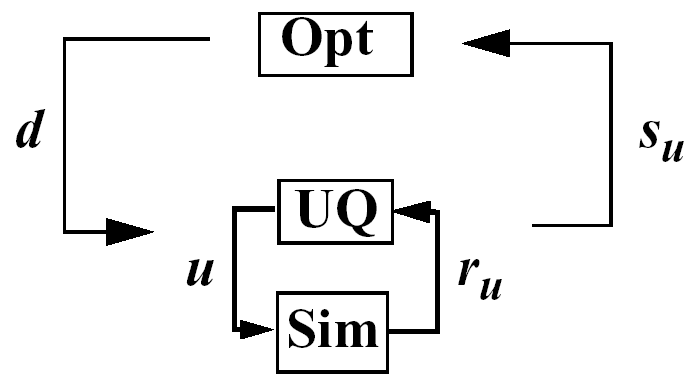
\includegraphics[scale=0.33]{images/nested_ouu}
  \caption{Formulation 1: Nested OUU.}
  \label{models:ex:figure08}
\end{figure}

Figure~\ref{models:ex:figure09} shows a DAKOTA input file for a nested
OUU example problem that is based on the textbook test problem. This
input file is named \texttt{dakota\_ouu1\_tb.in} in the
\texttt{Dakota/test} directory.  In this example, the objective
function contains two probability of failure estimates, and an
inequality constraint contains another probability of failure
estimate. For this example, failure is defined to occur when one of
the textbook response functions exceeds its threshold value. The
strategy keyword block at the top of the input file identifies this as
an OUU problem. The strategy keyword block is followed by the
optimization specification, consisting of the optimization method, the
continuous design variables, and the response quantities that will be
used by the optimizer. The mapping matrices used for incorporating UQ
statistics into the optimization response data are described in the
DAKOTA Reference Manual~\cite{RefMan}. The uncertainty quantification
specification includes the UQ method, the uncertain variable
probability distributions, the interface to the simulation code, and
the UQ response attributes. As with other complex DAKOTA input files,
the identification tags given in each keyword block can be used to
follow the relationships among the different keyword blocks.

\begin{figure}
  \centering
  \begin{bigbox}
    \begin{tiny}
      \verbatimtabinput[8]{dakota_ouu1_tb.in}
    \end{tiny}
  \end{bigbox}
  \caption{DAKOTA input file for the nested OUU example.}
  \label{models:ex:figure09}
\end{figure}

Latin hypercube sampling is used as the UQ method in this example
problem. Thus, each evaluation of the response functions by the
optimizer entails 50 Latin hypercube samples. In general, nested OUU
studies can easily generate several thousand function evaluations and
gradient-based optimizers may not perform well due to noisy or
insensitive statistics resulting from under-resolved sampling. These
observations motivate the use of surrogate-based approaches to OUU.

Other nested OUU examples in the \texttt{Dakota/test} directory
include \texttt{dakota\_ouu1\_tbch.in}, which adds an additional
interface for including deterministic data in the textbook OUU
problem, and\\ \texttt{dakota\_ouu1\_cantilever.in}, which solves the
cantilever OUU problem (see Section~\ref{additional:cantilever}) with
a nested approach. For each of these files, the ``\texttt{1}''
identifies formulation 1, which is short-hand for the nested approach.

% TO DO: combine with TR-SBOUU discussion?
\subsubsection{Surrogate-Based OUU (SBOUU)}\label{models:ex:ouu:sb}

Surrogate-based optimization under uncertainty strategies can be
effective in reducing the expense of OUU studies. Possible
formulations include use of a surrogate model at the optimization
level, at the uncertainty quantification level, or at both levels.
These surrogate models encompass both data fit surrogates (at the
optimization or UQ level) and model hierarchy surrogates (at the UQ
level only). Figure~\ref{models:ex:figure10} depicts the different
surrogate-based formulations where $\mathbf{\hat{r}_{u}}$ and
$\mathbf{\hat{s}_{u}}$ are approximate response functions and
approximate response statistics, respectively, generated from the
surrogate models.

\begin{figure}
  \centering
  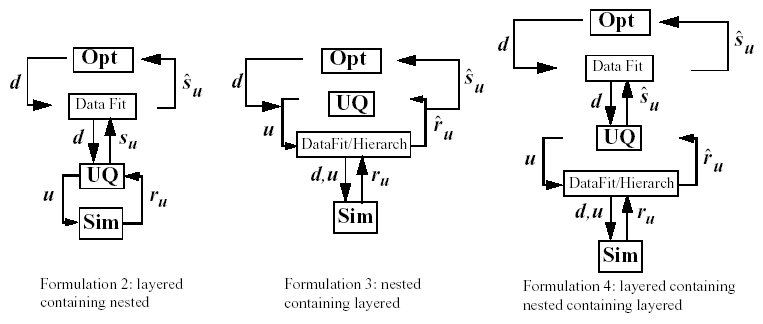
\includegraphics[scale=0.65]{images/sbouu}
  \caption{Formulations 2, 3, and 4 for Surrogate-based OUU.}
  \label{models:ex:figure10}
\end{figure}

SBOUU examples in the \texttt{Dakota/test} directory include
\texttt{dakota\_sbouu2\_tbch.in},\\ \texttt{dakota\_sbouu3\_tbch.in},
and \texttt{dakota\_sbouu4\_tbch.in}, which solve the textbook OUU
problem, and \texttt{dakota\_sbouu2\_cantilever.in},
\texttt{dakota\_sbouu3\_cantilever.in}, and\\
\texttt{dakota\_sbouu4\_cantilever.in}, which solve the cantilever OUU
problem (see Section~\ref{additional:cantilever}). For each of these
files, the ``\texttt{2},'' ``\texttt{3},'' and ``\texttt{4}'' identify
formulations 2, 3, and 4, which are short-hand for the ``layered
containing nested,'' ``nested containing layered,'' and ``layered
containing nested containing layered'' surrogate-based formulations,
respectively. In general, the use of surrogates greatly reduces the
computational expense of these OUU study. However, without restricting
and verifying the steps in the approximate optimization cycles,
weaknesses in the data fits can be exploited and poor solutions may be
obtained. The need to maintain accuracy of results leads to the use of
trust-region surrogate-based approaches.

\subsubsection{Trust-Region Surrogate-Based OUU (TR-SBOUU)}\label{models:ex:ouu:trsb}

The TR-SBOUU approach applies the trust region logic of deterministic
SBO (see Section~\ref{sbm:sblm}) to SBOUU. Trust-region verifications
are applicable when surrogates are used at the optimization level,
i.e., formulations 2 and 4. As a result of periodic verifications and
surrogate rebuilds, these techniques are more expensive than SBOUU;
however they are more reliable in that they maintain the accuracy of
results. Relative to nested OUU (formulation 1), TR-SBOUU tends to be
less expensive and less sensitive to initial seed and starting point.

TR-SBOUU examples in the \texttt{Dakota/test} directory include
\texttt{dakota\_trsbouu2\_tbch.in} and\\
\texttt{dakota\_trsbouu4\_tbch.in}, which solve the textbook OUU
problem, and\\ \texttt{dakota\_trsbouu2\_cantilever.in} and
\texttt{dakota\_trsbouu4\_cantilever.in}, which solve the cantilever
OUU problem (see Section~\ref{additional:cantilever}).

Computational results for several example problems are available
in~\cite{Eld02}.

\subsubsection{RBDO} \label{models:ex:ouu:rbdo}

Bi-level and sequential approaches to reliability-based design
optimization (RBDO) and their associated sensitivity analysis
requirements are described in the Optimization Under Uncertainty
chapter of the Theory Manual.

A number of bi-level RBDO examples are provided in \texttt{Dakota/test}.
The \texttt{dakota\_rbdo\_cantilever.in},
\texttt{dakota\_rbdo\_short\_column.in}, and
\texttt{dakota\_rbdo\_steel\_column.in} input files solve the
cantilever (see Section~\ref{additional:cantilever}), short column
(see Section~\ref{additional:short_column}), and steel column (see
Section~\ref{additional:steel_column}) OUU problems using a bi-level
RBDO approach employing numerical design gradients.  The 
\texttt{dakota\_rbdo\_cantilever\_analytic.in} and
\texttt{dakota\_rbdo\_short\_column\_analytic.in} input files solve
the cantilever and short column OUU problems using a bi-level RBDO
approach with analytic design gradients and first-order limit state
approximations.  The \texttt{dakota\_rbdo\_cantilever\_analytic2.in},
\texttt{dakota\_rbdo\_short\_column\_analytic2.in}, and
\texttt{dakota\_rbdo\_steel\_column\_analytic2.in} input files also
employ analytic design gradients, but are extended to employ
second-order limit state approximations and integrations.

Sequential RBDO examples are also provided in \texttt{Dakota/test}.  
The \texttt{dakota\_rbdo\_cantilever\_trsb.in} and
\texttt{dakota\_rbdo\_short\_column\_trsb.in} input files solve 
the cantilever and short column OUU problems using a first-order
sequential RBDO approach with analytic design gradients and
first-order limit state approximations.  The
\texttt{dakota\_rbdo\_cantilever\_trsb2.in},
\texttt{dakota\_rbdo\_short\_column\_trsb2.in}, and 
\texttt{dakota\_rbdo\_steel\_column\_trsb2.in} input files 
utilize second-order sequential RBDO approaches that employ
second-order limit state approximations and integrations (from
analytic limit state Hessians with respect to the uncertain variables)
and quasi-Newton approximations to the reliability metric Hessians
with respect to design variables.

\subsubsection{Stochastic Expansion-Based Design Optimization} \label{models:ex:ouu:sebdo}

For stochastic expansion-based approaches to optimization under
uncertainty, bi-level, sequential, and multifidelity approaches and
their associated sensitivity analysis requirements are described in
the Optimization Under Uncertainty chapter of the Theory Manual.

In \texttt{Dakota/test}, the \texttt{dakota\_pcbdo\_cantilever.in},
\texttt{dakota\_pcbdo\_rosenbrock.in},\\
\texttt{dakota\_pcbdo\_short\_column.in}, and
\texttt{dakota\_pcbdo\_steel\_column.in} input files solve 
cantilever (see Section~\ref{additional:cantilever}), Rosenbrock,
short column (see Section~\ref{additional:short_column}), and steel
column (see Section~\ref{additional:steel_column}) OUU problems using
a bi-level polynomial chaos-based approach, where the statistical
design metrics are reliability indices based on moment projection
(i.e., Eqs.~\ref{eq:mv_ria_cdf}-\ref{eq:mv_ria_ccdf}).  The test
matrix in the former three input files evaluate design gradients of
these reliability indices using several different approaches: analytic
design gradients based on a PCE formed over only over the random
variables (Eqs.~\ref{eq:dmuR_ds_unc_pce}-\ref{eq:dsigR_ds_unc_pce}),
analytic design gradients based on a PCE formed over all variables
(differentiation of
Eqs.~\ref{eq:muR_comb_pce}-\ref{eq:sigR_comb_pce}), numerical design
gradients based on a PCE formed only over the random variables, and
numerical design gradients based on a PCE formed over all variables.
In the cases where the expansion is formed over all variables, only a
single PCE construction is required for the complete PCBDO process,
whereas the expansions only over the random variables must be
recomputed for each change in design variables.  Sensitivities for
``augmented'' design variables (which are separate from and augment
the random variables) may be handled using either analytic approach;
however, sensitivities for ``inserted'' design variables (which define
distribution parameters for the random variables) must be handled
using Eqs.~\ref{eq:dmuR_ds_unc_pce}-\ref{eq:dsigR_ds_unc_pce} where
$\frac{dR}{ds}$ is calculated as $\frac{dR}{dx} \frac{dx}{ds}$.
Additional test input files include:
\begin{itemize}
\item \texttt{dakota\_scbdo\_cantilever.in}, 
\texttt{dakota\_scbdo\_rosenbrock.in}, \\
\texttt{dakota\_scbdo\_short\_column.in}, and
\texttt{dakota\_scbdo\_steel\_column.in} input files solve 
cantilever, Rosenbrock, short column, and steel column OUU problems
using a bi-level stochastic collocation-based approach.

\item \texttt{dakota\_pcbdo\_cantilever\_trsb.in},
\texttt{dakota\_pcbdo\_rosenbrock\_trsb.in}, \\
\texttt{dakota\_pcbdo\_short\_column\_trsb.in}, 
\texttt{dakota\_pcbdo\_steel\_column\_trsb.in},\\
\texttt{dakota\_scbdo\_cantilever\_trsb.in}, 
\texttt{dakota\_scbdo\_rosenbrock\_trsb.in}, \\
\texttt{dakota\_scbdo\_short\_column\_trsb.in}, and
\texttt{dakota\_scbdo\_steel\_column\_trsb.in} input files solve 
cantilever, Rosenbrock, short column, and steel column OUU problems
using sequential polynomial chaos-based and stochastic
collocation-based approaches.

\item \texttt{dakota\_pcbdo\_cantilever\_mf.in},
\texttt{dakota\_pcbdo\_rosenbrock\_mf.in}, \\
\texttt{dakota\_pcbdo\_short\_column\_mf.in}, 
\texttt{dakota\_scbdo\_cantilever\_mf.in}, \\
\texttt{dakota\_scbdo\_rosenbrock\_mf.in}, and
\texttt{dakota\_scbdo\_short\_column\_mf.in} input files solve 
cantilever, Rosenbrock, and short column OUU problems
using multifidelity polynomial chaos-based and stochastic
collocation-based approaches.
\end{itemize}


\subsubsection{Epistemic OUU} \label{models:ex:ouu:epistemic}

An emerging capability is optimization under epistemic uncertainty.
As described in the Nested Model section of the Reference
Manual~\cite{RefMan}, epistemic and mixed aleatory/epistemic
uncertainty quantification methods generate lower and upper interval
bounds for all requested response, probability, reliability, and
generalized reliability level mappings.  Design for robustness in the
presence of epistemic uncertainty could simply involve minimizing the
range of these intervals (subtracting lower from upper using the
nested model response mappings), and design for reliability in the
presence of epistemic uncertainty could involve controlling the worst
case upper or lower bound of the interval.

We now have the capability to perform epistemic analysis by 
using interval optimization on the ``outer loop'' to calculate bounding 
statistics of the aleatory uncertainty on the ``inner loop.''  
Preliminary studies~\cite{Eld09b} have shown this approach is more efficient 
and accurate than nested sampling (which was described in 
Section~\ref{models:ex:sop}).  This approach uses 
an efficient global optimization method for the outer loop and 
stochastic expansion methods (e.g. polynomial chaos or stochastic 
collocation on the inner loop).  The interval optimization is described in 
Section~\ref{uq:interval}.  Example input files demonstrating 
the use of interval estimation for epistemic analysis, 
specifically in epistemic-aleatory nesting, are: 
\texttt{dakota\_uq\_cantilever\_sop\_exp.in}, and
\texttt{dakota\_short\_column\_sop\_exp.in}. 

\subsection{Surrogate-Based Uncertainty Quantification} \label{models:ex:sbuq}

Many uncertainty quantification (UQ) methods are computationally costly. 
For example, sampling often requires many function evaluations to obtain 
accurate estimates of moments or percentile values of an output distribution.  
One approach to overcome the computational cost of sampling is to 
evaluate the true function (e.g. run the analysis driver) on a fixed, small
set of samples, use these sample evaluations to 
create a response surface approximation (e.g. a surrogate model or meta-model)
of the underlying ``true'' function, then perform random sampling (using 
thousands or millions of samples) on the approximation to obtain estimates 
of the mean, variance, and percentiles of the response. 

This approach, called ``surrogate-based uncertainty quantification'' 
is easy to do in DAKOTA, and one can set up input files to compare the 
results using no approximation (e.g. determine the mean, variance, and 
percentiles of the output directly based on the initial sample values) 
with the results obtained by sampling a variety of surrogate approximations.  
Example input files of a standard UQ analysis based on sampling alone vs. 
sampling a surrogate are shown in the \texttt{dakota\_uq\_sampling.in} and 
\texttt{dakota\_surr\_uq.in} in the \texttt{Dakota/examples/methods}
directory. 

Note that one must exercise some caution when using surrogate-based methods 
for uncertainty quantification. In general, there is not a single, 
straightforward approach to incorporate the error of the surrogate fit 
into the uncertainty estimates of the output produced by sampling the surrogate.
Two references which discuss some of the related 
issues are~\cite{Giu06} and~\cite{Swi06}. The first reference shows that 
statistics of a response based on a surrogate model were less accurate, and 
sometimes biased, for surrogates constructed on very small sample sizes.  
In many cases, however,~\cite{Giu06} shows that surrogate-based UQ performs 
well and sometimes generates more accurate estimates of statistical
quantities on the output.  The second reference goes into more detail 
about the interaction between sample type and response surface type (e.g., 
are some response surfaces more accurate when constructed on a particular 
sample type such as LHS vs. an orthogonal array?) In general, there is not 
a strong dependence of the surrogate performance with respect to sample type, 
but some sample types perform better with respect to some metrics and not 
others (for example, a Hammersley sample may do well at lowering root mean 
square error of the surrogate fit but perform poorly at lowering the maximum 
absolute deviation of the error).  Much of this work is empirical and 
application dependent.  If you choose to use surrogates in uncertainty 
quantification, we strongly recommend trying a variety of surrogates 
and examining diagnostic goodness-of-fit metrics. 
